\documentclass[final]{beamer}

\usepackage[scale=1.24]{beamerposter} % Use the beamerposter package for laying out the poster

\usepackage{siunitx}

\usetheme{confposter} % Use the confposter theme supplied with this template

\setbeamercolor{block title}{fg=nblue,bg=white} % Colors of the block titles
\setbeamercolor{block body}{fg=black,bg=white} % Colors of the body of blocks
\setbeamercolor{block alerted title}{fg=white,bg=dblue!70} % Colors of the highlighted block titles
\setbeamercolor{block alerted body}{fg=black,bg=dblue!10} % Colors of the body of highlighted blocks
% Many more colors are available for use in beamerthemeconfposter.sty

\usepackage[skins]{tcolorbox}
% a "sub-block" (plain block-within-block (second-level header))
\newenvironment{subblock}[1]{
  \setbeamertemplate{block begin}
  {
    \setbeamercolor{block title}{fg=nblue!90} % @TODO defer to beamercolortheme
    \par\vskip\medskipamount
    \begin{beamercolorbox}[colsep*=0ex,dp={2ex}]{block title}
      \vskip-0.5cm
      \begin{tikzpicture}[every node/.style={inner sep=0}]
        \node (titlenode) at (0.1cm, 0) {\usebeamerfont{block title}\normalsize\insertblocktitle};
        \tcbsetmacrotowidthofnode{\titlewidth}{titlenode}
        \tcbsetmacrotoheightofnode{\titleheight}{titlenode}
        \shade [inner color=nblue!16!black!24,outer color=white]
        (-\titlewidth/2,-\titleheight/2) rectangle ++({1.1*\titlewidth+0.1cm},-0.2cm);
      \end{tikzpicture}
    \end{beamercolorbox}
    {\parskip0pt\par}
    \ifbeamercolorempty[bg]{block title}
    {}
    {\ifbeamercolorempty[bg]{block body}{}{\nointerlineskip\vskip-0.5pt}}
    \usebeamerfont{block body}
    \vskip-0.5cm
    \begin{beamercolorbox}[colsep*=0ex,vmode]{block body}
      \justifying
    }
    \setbeamertemplate{block end}
    {
    \end{beamercolorbox}
    \vskip\smallskipamount
  }
  \begin{block}{{\normalsize #1}}
  }{\end{block}}

\newlength{\sepwid}
\newlength{\colonewid}
\newlength{\coltwowid}
\newlength{\colthreewid}
\setlength{\paperwidth}{48in} % A0 width: 46.8in
\setlength{\paperheight}{36in} % A0 height: 33.1in
\setlength{\sepwid}{0.024\paperwidth} % Separation width (white space) between columns
\setlength{\colonewid}{0.29\paperwidth} % Width of column one
\setlength{\coltwowid}{0.324\paperwidth} % Width of column two
\setlength{\colthreewid}{0.29\paperwidth} % Width of one column
\setlength{\topmargin}{-0.5in} % Reduce the top margin size
% -----------------------------------------------------------

\usepackage{graphicx}  % Required for including images
\usepackage{booktabs} % Top and bottom rules for tables
\usepackage{tikz}
\usetikzlibrary{
  arrows,
  calc,
  decorations.pathmorphing,
  decorations.pathreplacing,
  decorations.markings,
  fadings,
  positioning,
  shapes,
  arrows.meta
}
\usepgfmodule{oo}

% --------------------------------------------------------------------------------
%	TITLE SECTION
% --------------------------------------------------------------------------------

\def\realtitle{A next-generation trapped ion quantum computing system}

\title{%
  \texorpdfstring{%
    \makebox[\linewidth]{%
      \makebox[0pt][l]{%
        \raisebox{\dimexpr-\height+0.5\baselineskip}[0pt][0pt]
        {
          \begin{tikzpicture}
            \node at (0, 0) {
\includegraphics[width=17cm]{imgs/logos/Duke}};
            \node at (0, -4.5) {
\includegraphics[width=17cm]{imgs/logos/UMD}};

            \node at (12.5, 0) {
\includegraphics[width=4cm]{imgs/logos/ARL}};
            \node at (16, -4) {
\includegraphics[width=4cm]{imgs/logos/IARPA}};
          \end{tikzpicture}
        }% Left logo
      }\hfill
      \makebox[0pt]{\textcolor{dblue}{\realtitle}}%
      \hfill\makebox[0pt][r]{%
        \raisebox{\dimexpr-\height+0.5\baselineskip}[0pt][0pt]
        {
          \begin{tikzpicture}
            \node at (0, 0) {
\includegraphics[width=7.5cm]{imgs/logos/NIST}};
            \node at (8.5, 0) {
\includegraphics[width=7.5cm]{imgs/logos/Sandia}};
            \node at (17.75, 0) {
\includegraphics[width=9cm]{imgs/logos/L3Harris}};
            \node at (3.25, -4) {
\includegraphics[width=9cm]{imgs/logos/ColdQuanta}};
            \node at (15.25, -4) {
\includegraphics[width=9cm]{imgs/logos/AOSense}};
          \end{tikzpicture}
        }% Right logo
      }%
    }%
  }
  {\realtitle}} % Poster title

\author{Yichao Yu \inst{1}, Liudmila Zhukas \inst{1}, Lei Feng \inst{1,2},
  Marko Cetina \inst{1,2}, Crystal Noel \inst{1,2},\\
  Debopriyo Biswas \inst{1,2}, Andrew Risinger \inst{2},
  Alexander Kozhanov \inst{1}, Christopher R Monroe \inst{1,2,3}}
\institute{\inst{1} Duke Quantum Center, Duke University
  \inst{2} Joint Quantum Institute, University of Maryland
  \inst{3} IonQ, Inc.}

\ifpdf
  % Ensure reproducible output
  \pdfinfoomitdate=1
  \pdfsuppressptexinfo=-1
  \pdftrailerid{}
  \hypersetup{
    pdfcreator={},
    pdfproducer={}
  }
\fi

\begin{document}

\addtobeamertemplate{block end}{}{\vspace*{2ex}} % White space under blocks
\addtobeamertemplate{block alerted end}{}{\vspace*{2ex}} % White space under highlighted (alert) blocks

\setlength{\belowcaptionskip}{2ex} % White space under figures
\setlength\belowdisplayshortskip{2ex} % White space under equations

\definecolor{trapyellow}{HTML}{ffe0a5}
\definecolor{semgray}{HTML}{cccccc}

\begin{frame}[t] % The whole poster is enclosed in one beamer frame
  \begin{columns}[t]
    \begin{column}{\sepwid}\end{column} % Empty spacer column
    \begin{column}{\colonewid} % The first column
      \vspace{-0.8cm}
      \begin{block}{\textbf{E}rror-corrected \textbf{U}niversal \textbf{R}econfigurable
          \textbf{I}on-trap \textbf{Q}uantum \textbf{A}rchetype}
        \begin{center}
          \vspace{-1cm}
          \begin{tikzpicture}
            \begin{scope}[shift={(-7.5,0)}]
              \node[above] at (0, 0) {$1^{\text{st}}$ Generation};
              \node[below] at (0, 0) {
                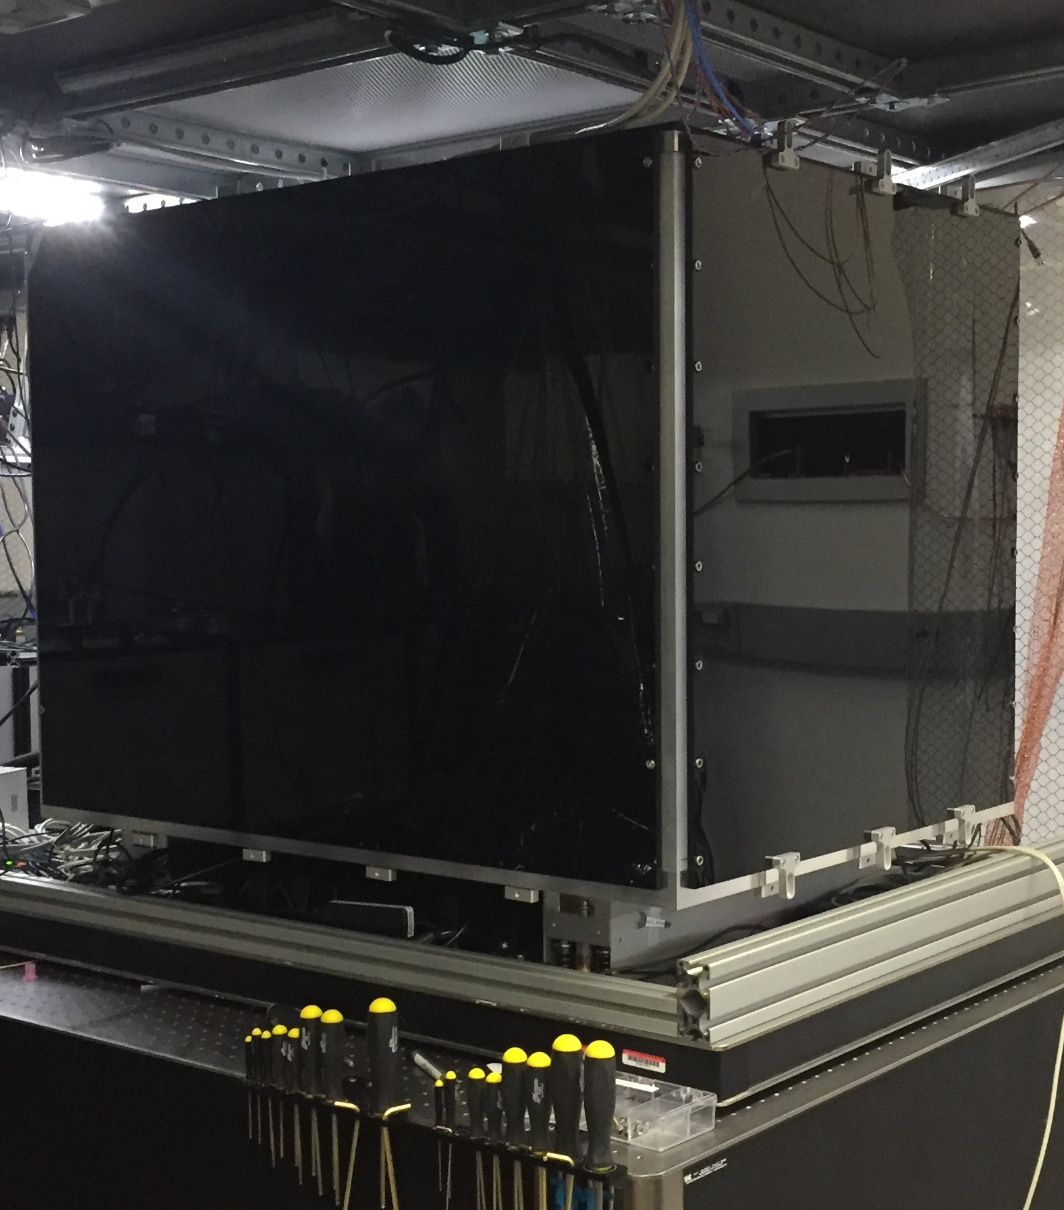
\includegraphics[width=12.5cm]{imgs/Breadboard_box}
              };
              \node[below,text width=12.5cm,align=left] at (-0.15, -1.85) {
                \setbeamercolor{itemize/enumerate body}{fg=white}
                \begin{itemize}
                \item 15-24 usable qubits
                \item High fidelity single ($99.9\ \%$) and two-qubit ($99\ \%$) gates
                \item Universal reconfigurable
                \item Remote operations
                \end{itemize}
              };
            \end{scope}
            \begin{scope}[shift={(7.5,0)}]
              \node[above] at (0, 0) {$2^{\text{nd}}$ Generation};
              \node[below] at (0, -0.7) {
                \includegraphics[width=17cm]{imgs/LabPicture}
              };
            \end{scope}
          \end{tikzpicture}
        \end{center}
      \end{block}
      \vspace{-0.7cm}

      \begin{block}{Vacuum System}
        \begin{center}
          \begin{columns}
            \column{16cm}
            \begin{itemize}
            \item Vacuum fired components
            \item Reduce ion-chain reordering rate
            \item $10^{-11}\ \mathrm{Torr}$ measured pressure
            \end{itemize}
            \begin{center}
              \includegraphics[width=10cm]{imgs/Reorder_rate.png}\\
              {\footnotesize 15-ion chain reordering
                in $1^{\text{st}}$ gen EURIQA system.}\\
              {\footnotesize Consistent with $10^{-10}\ \mathrm{Torr}$.}\\
              {\scriptsize Cetina, et al.}
            \end{center}
            \column{13cm}
            \includegraphics[width=12cm]{imgs/Vacuum_stack_photo.png}
          \end{columns}
        \end{center}
      \end{block}

      \begin{block}{Phoenix Surface Trap}
        \begin{tikzpicture}
          \begin{scope}[scale=2.5, shift={(3, -4)}]
            \node at (3, 2) {\includegraphics[width=12cm]{imgs/Phoenix}};
            \fill[semgray,opacity=0.6] (1.8, 2.115) -- (-4.65, -0.3875)
            -- (-0.35, -3.6125) -- (1.9, 2.115) -- cycle;
            \fill[trapyellow,opacity=0.6] (2.85, 2.115) -- (0.9, -1) -- (5.7, -1)
            -- (3.15, 2.115) -- cycle;
            \node at (3.3, -2) {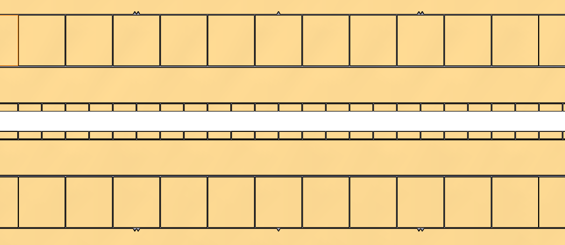
\includegraphics[width=12cm]{imgs/Phoenix_quantum}};
            \node at (-2.5, -2) {\includegraphics[width=10.75cm]{imgs/Phoenix_Loading_SEM}};
          \end{scope}
          \node[below,text width=16cm,align=left] at (0, 0) {
            \begin{itemize}
            \item Better metallization
              \begin{itemize}
              \item Reducing noise
              \item Less charging/photovoltaic effect
              \end{itemize}
              \begin{center}
                {\small 30 quanta/s heating rate @ 3 MHz}\\
                {\scriptsize Measured by Sandia}
              \end{center}
            \item Segmented outer electrodes
            \item Better and faster ion loading
            \end{itemize}
          };
          \node at (7.5, -23) {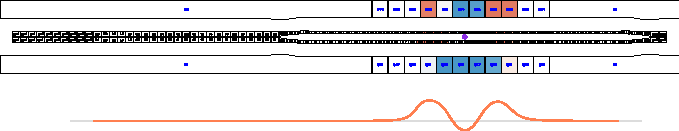
\includegraphics[width=30cm]{imgs/center_voltage.pdf}};
          \fill[semgray,opacity=0.6] (13.03, -21.72)
            -- (15, -26.25) -- (22.5, -26.25) -- cycle;
          \fill[semgray!90!blue,opacity=0.6] (-2.47, -21.72)
            -- (0, -26.25) -- (-7.5, -26.25) -- cycle;
          \node at (-3.75, -30) {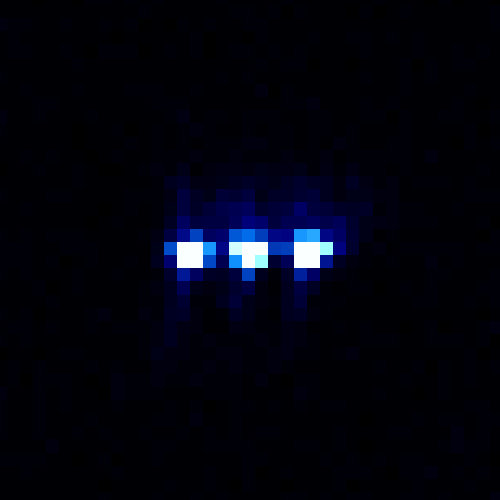
\includegraphics[width=7.5cm]{imgs/three_ions.png}};
          \node at (18.75, -30) {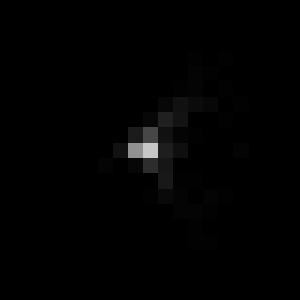
\includegraphics[width=7.5cm]{imgs/quantum_ion.png}};
          \node[below,text width=14.5cm,align=left] at (7.5, -26.25) {
            \begin{itemize}
            \item Trapped chain of ions
            \item Imaged ions in quantum region
            \item Shuttled chain of ions
            \end{itemize}
          };
        \end{tikzpicture}
      \end{block}
    \end{column} % End of the first column

    \begin{column}{\sepwid}
      \begin{center}
        {\color{gray}\rule{3pt}{\textheight}}
      \end{center}
    \end{column} % Empty spacer column

    \begin{column}{\coltwowid}
      \begin{block}{Raman System}
        \begin{center}
          \vspace{-1cm}
          \begin{tikzpicture}[scale=2.5]
            \begin{scope}[shift={(-3.5, 0)}]
              \node[align=center] at (-1.5, 3.25)
              {\usebeamercolor[fg]{frametitle}{\bf 1$^{\text{st}}$ gen}};
              \node[align=center] at (0, 1.75)
              {\includegraphics[width=11.5cm]{imgs/Breadboard_Raman.png}};

              \begin{scope}[shift={(1.75, 2.8)}]
                \draw[->,blue!80!black,line width=5,>=stealth] (-1.9, -2.5) --
                node[below] {$\bf k_{glob}$} (-0.1, -2.5);
                \draw[<-,blue!80!black,line width=5,>=stealth] (0, -2.4) --
                node[below,sloped] {$\bf k_{ind}$} (0, -0.6);
                \draw[->,green!60!black,line width=5,>=stealth] (-1.9, -2.4) --
                node[above,sloped] {$\bf \Delta k$} (-0.1, -0.6);
              \end{scope}
            \end{scope}

            \draw[->,red!60!black,line width=0.7] (0, 0) --
            node[sloped,font=\small,align=center]
            {Dominant\\E field noise} (0, 2);

            \begin{scope}[shift={(3.5, 0)}]
              \node[align=center] at (-1.5, 3.25)
              {\usebeamercolor[fg]{frametitle}{\bf 2$^{\text{nd}}$ gen}};
              \node[align=center] at (0, 1.75)
              {\includegraphics[width=11.5cm]{imgs/Brassboard_Raman.png}};

              \begin{scope}[shift={(0, 2.8)}]
                \draw[->,blue!80!black,line width=5,>=stealth] (-1.9, -2.5) --
                node[below] {$\bf k_{glob}$} (-0.1, -2.5);
                \draw[->,blue!80!black,line width=5,>=stealth] (1.9, -2.5) --
                node[below] {$\bf k_{ind}$} (0.1, -2.5);
                \draw[->,green!60!black,line width=5,>=stealth] (-1.9, -2.3) --
                node[above,sloped] {$\bf \Delta k$} (1.9, -2.3);
              \end{scope}
            \end{scope}

            \begin{scope}[shift={(0, -3.5)}]
              \node at (0, 0) {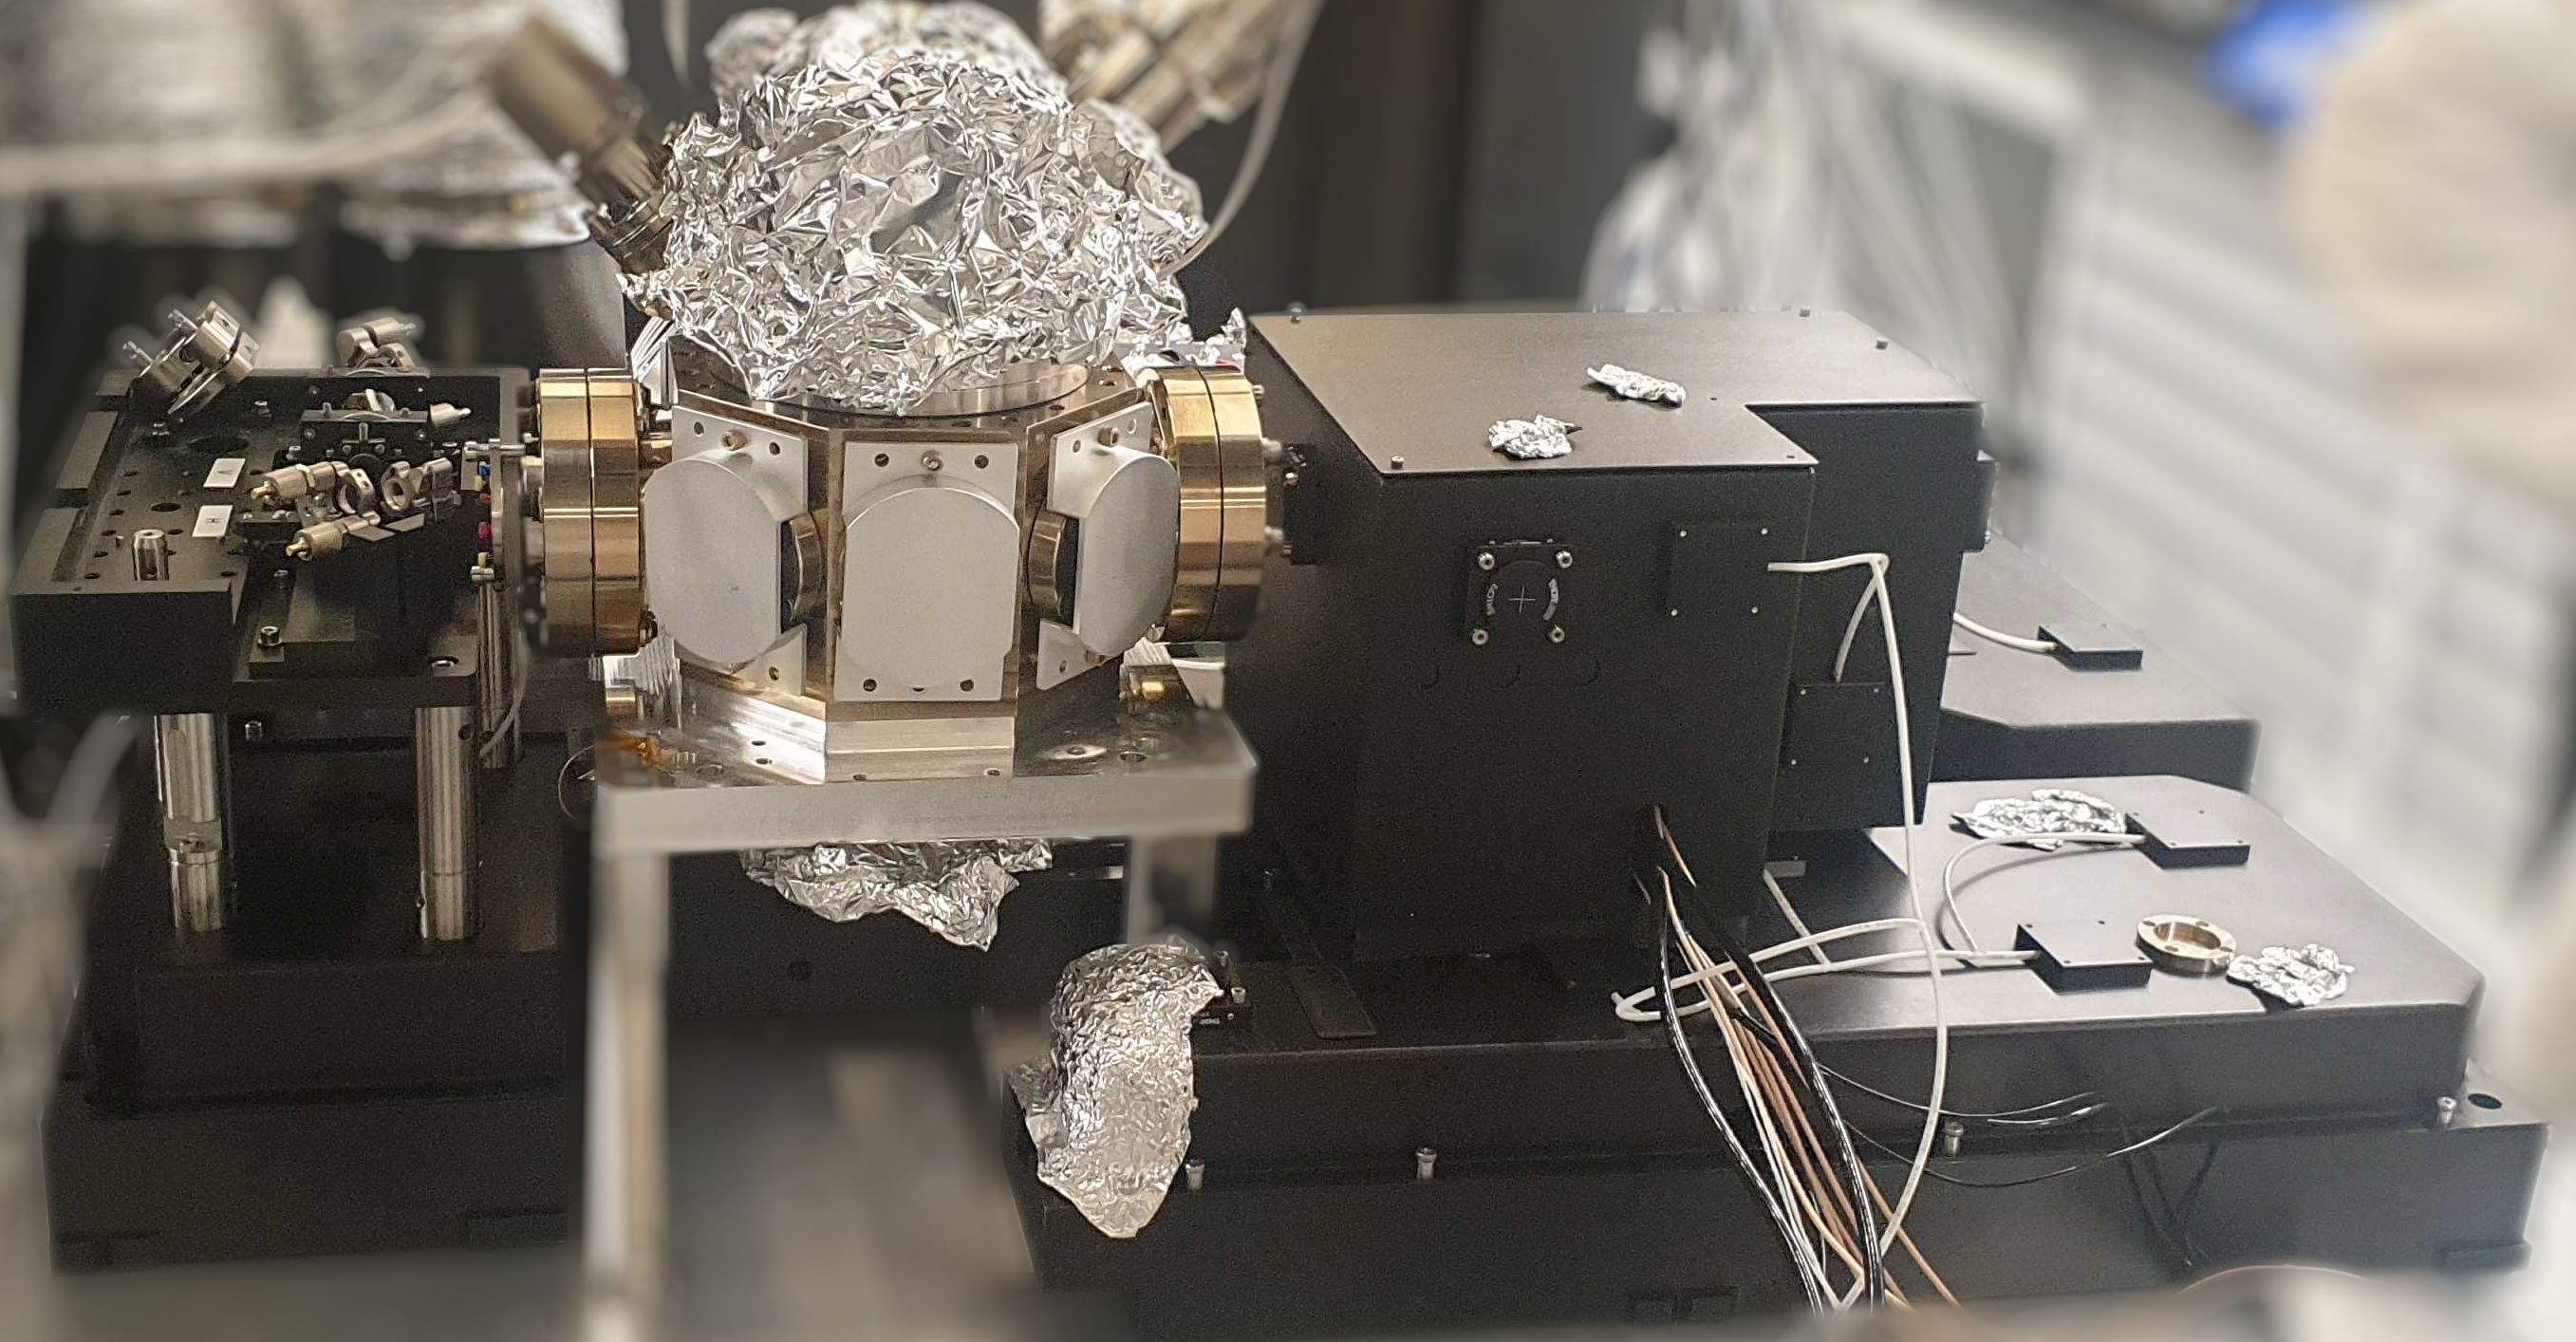
\includegraphics[width=26cm]{imgs/Harris_optics.png}};
              \node at (3.7, 2) {
\includegraphics[width=7cm]{imgs/logos/L3Harris.png}};

              \node[align=center] at (3, -3.25)
              {
\includegraphics[height=1.25cm]{imgs/Global_beam.png}};
              \fill[semgray,opacity=0.6] (-0.07, 0.65)
              -- (1.038, -3) -- (4.962, -3) -- cycle;
              \node[below] at (3, -3 - 0.8) {Global Raman Beam};
              \begin{scope}[shift={(-3, -3)}]
                \begin{scope}[scale=0.5]
                  \node[align=center] at (0, -0.5)
                  {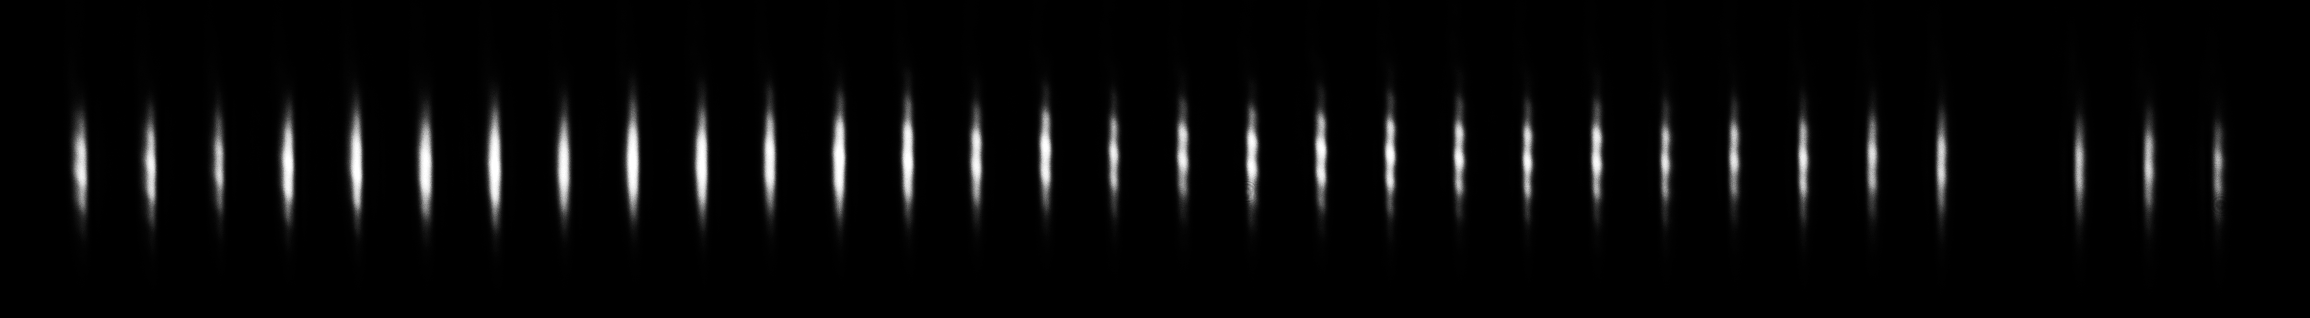
\includegraphics[height=1.875cm]{imgs/Individual_beam.png}};
                  \draw[dotted,line width=1,gray] (-1.17, -0.5) -- (-1.17, -1.6);
                  \draw[dotted,line width=1,gray] (-1.49, -0.5) -- (-1.49, -1.6);
                  \draw[<-,>=stealth,line width=1] (-1.49, -1.5) -- ++(-0.8, 0);
                  \draw[<-,>=stealth,line width=1] (-1.17, -1.5) -- ++(0.8, 0);
                  \node[below] at (-1.33, -1.6) {$4.5\mathrm{\mu m}$};
                \end{scope}
                \node[below] at (0, -1.25) {Individual Raman Beams};
              \end{scope}
              \fill[semgray,opacity=0.6] (-3, 0.6)
              -- (-5.724, -2.875) -- (-0.276, -2.875) -- cycle;
            \end{scope}

          \end{tikzpicture}
        \end{center}
      \end{block}
      \begin{block}{Miniaturized 369/399/780/935nm Beam Path}
        \begin{center}
          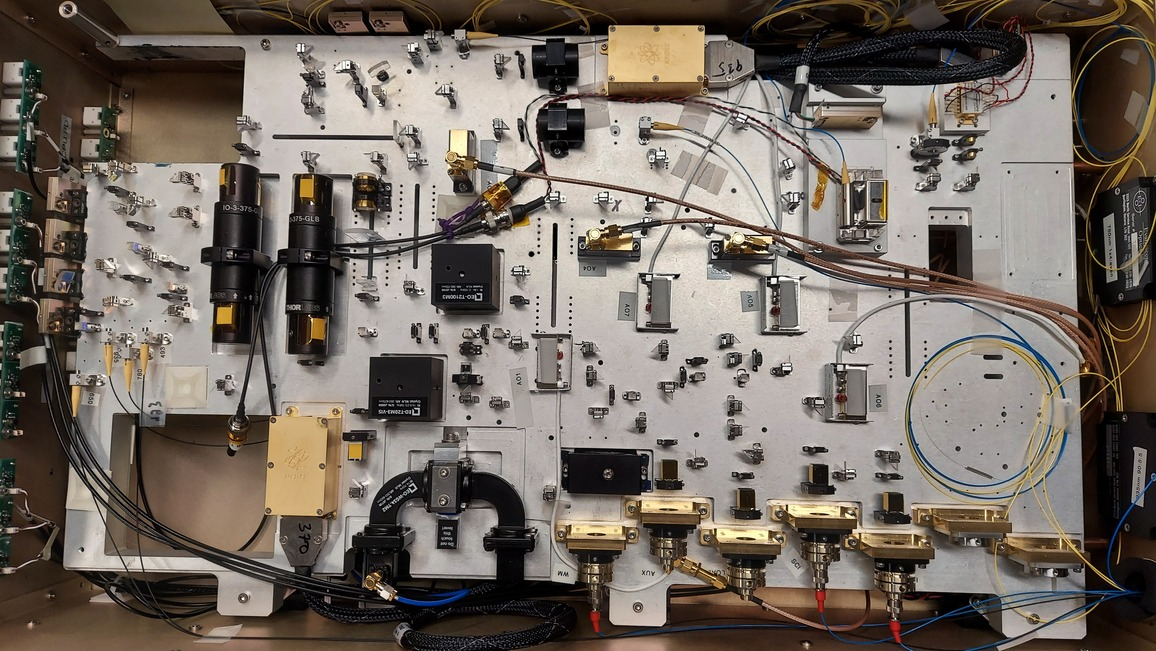
\includegraphics[height=11.2cm]{imgs/AOSense_internal.jpg}
          \hspace{2.5cm}
          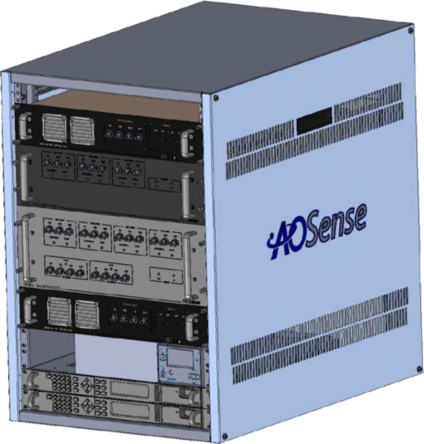
\includegraphics[height=10.8cm]{imgs/AOSense_external.png}
        \end{center}
      \end{block}
      \begin{block}{Control System}
        \vspace{-1cm}
        \begin{center}
          \begin{columns}[t]
            \begin{column}{0.36\coltwowid}
              \begin{subblock}{ARTIQ}
                \begin{itemize}
                \item Artiq software
                \item Sinara hardware
                \end{itemize}
                \vspace{0.3cm}
                \begin{center}
                  \includegraphics[width=12cm]{imgs/artiq_hardware.png}
                \end{center}
              \end{subblock}
              \begin{subblock}{RFSoC/Pentek}
                \begin{itemize}
                \item integrated pulse-level control
                \item phase synchronization
                \end{itemize}
                \begin{center}
                  \includegraphics[width=12cm]{imgs/pentek.png}
                \end{center}
              \end{subblock}
            \end{column}
            \begin{column}{0.54\coltwowid}
              \begin{subblock}{Duke Artiq Extensions}
                \begin{itemize}
                \item modular control software
                \item system code organization
                \end{itemize}
                \vspace{0.7cm}
                \begin{center}
                  \includegraphics[width=19cm]{imgs/dax.pdf}
                \end{center}
              \end{subblock}
            \end{column}
          \end{columns}
        \end{center}
      \end{block}
    \end{column} % End of the second column

    \begin{column}{\sepwid}
      \begin{center}
        {\color{gray}\rule{3pt}{\textheight}}
      \end{center}
    \end{column} % Empty spacer column

    \begin{column}{\colthreewid} % The third column
      \begin{block}{Imaging System}
        \vspace{0.5cm}
        \begin{center}
          \begin{tikzpicture}
            \node at (0, 1) {\includegraphics[width=33cm]{imgs/imaging_system.png}};
            \node[text width=28cm,align=left] at (-3.5, -12.5) {
              \begin{itemize}
              \item Imaging system for 32 ions, fixed 4.5 \unit{\micro\meter} spacing between ions
              \item Two stage imaging system with a total magnification of 27
              \item Minimized instrumental crosstalk by coupling fluorescence from each ion to the individual PMT module (Hamamatsu, H10682-210)
              \item PhotonGear optical lens design (0.63 NA)\\
                mounted on PI Hexapod for precise positioning
              \item Zemax simulations: the resulting Strehl ratio\\
                is >~0.95 for all 32 ions in the chain
              \end{itemize}
            };
            \node at (-6.5, -27) {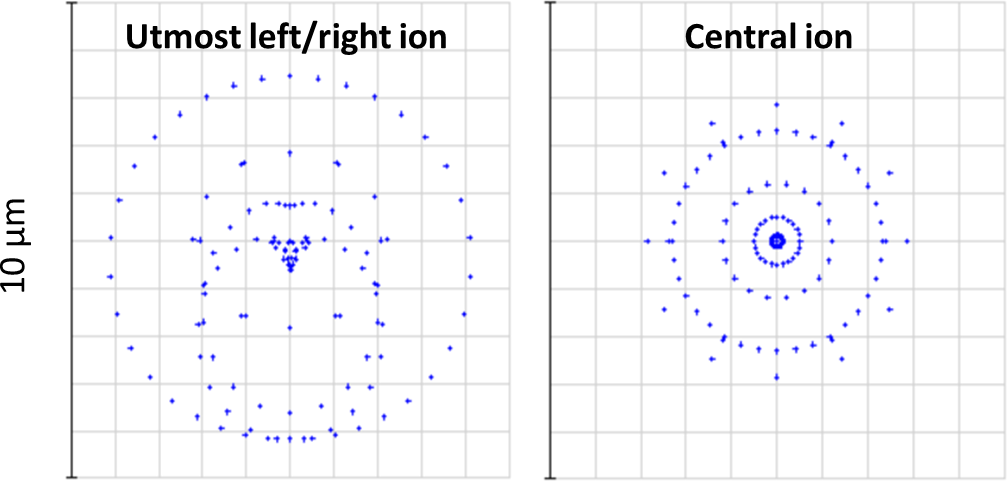
\includegraphics[width=20cm]{imgs/zeemax_sim.png}};
            \node at (11.5, -24) {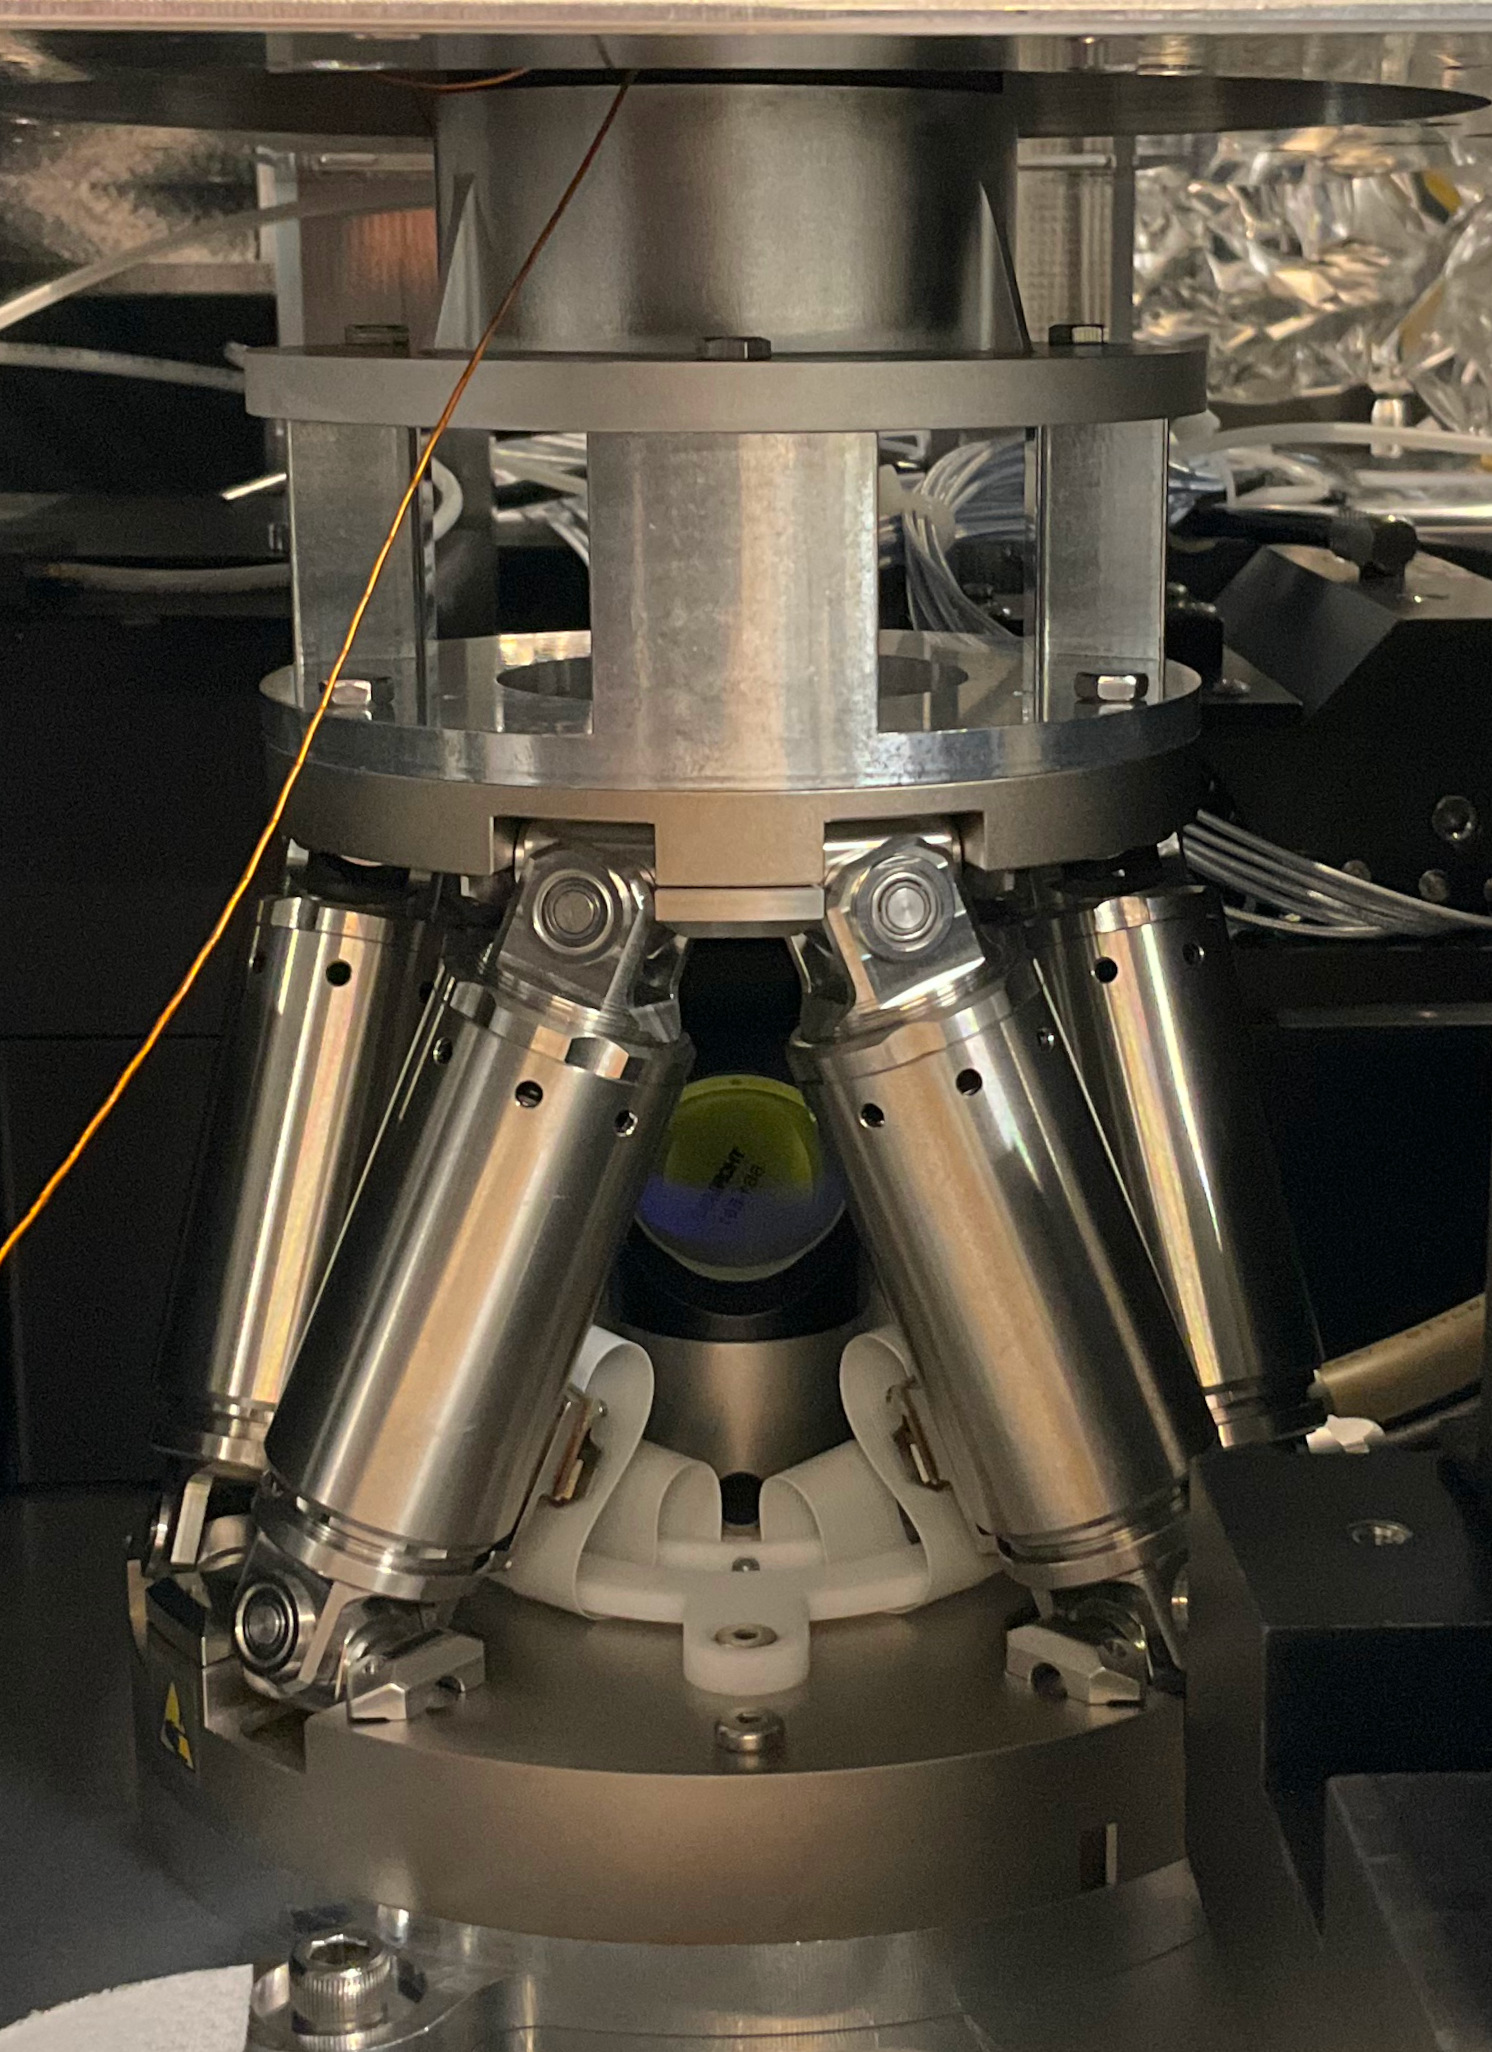
\includegraphics[width=12cm]{imgs/hexapod.jpg}};
          \end{tikzpicture}
        \end{center}
        \vspace{0.5cm}
      \end{block}

      \begin{block}{Applications}
        \vspace{1cm}
        \begin{tikzpicture}
          \node at (0, -0.5) {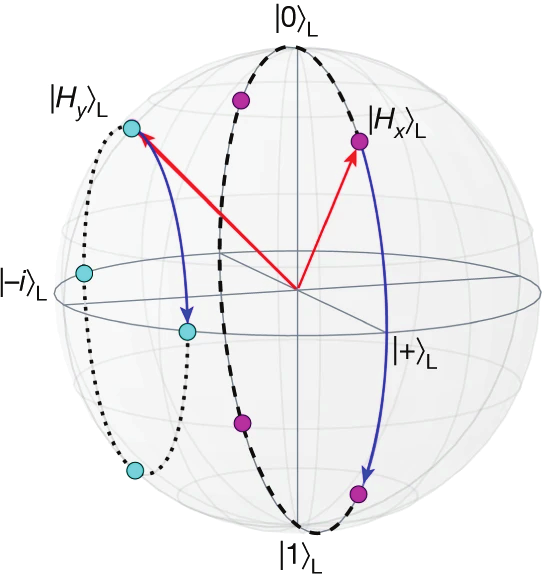
\includegraphics[width=9cm]{imgs/app1.png}};
          \node at (24, -5.1) {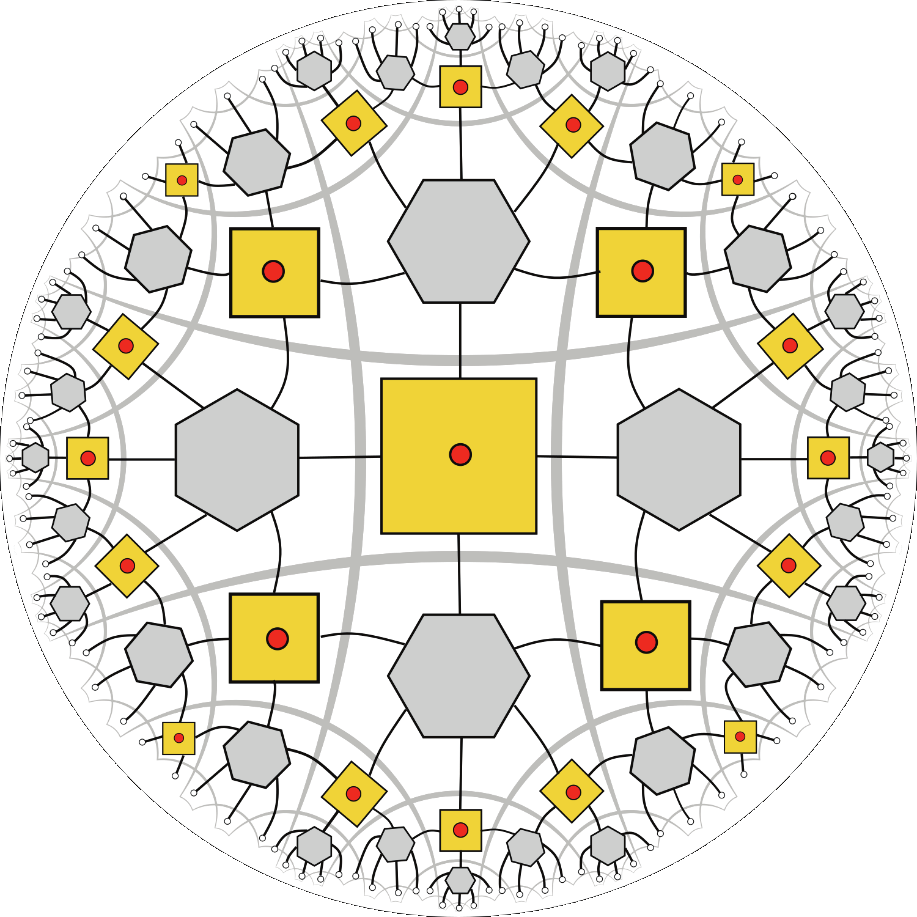
\includegraphics[width=11.6cm]{imgs/app2.png}};
          \node[below,text width=15cm,align=left] at (12, 4.5) {
            \begin{itemize}
            \item Universal Quantum Computer
            \item 20+ qubits and high fidelity
            \item Quantum simulations of many body physics
            \item Quantum chemistry
            \item Quantum gravity
            \item Nuclear theory
            \item Quantum Error\\
              Correction
            \end{itemize}
          };
          \node at (13, -16) {
            \includegraphics[width=10.5cm]{imgs/app4.pdf}
            \includegraphics[width=10.5cm]{imgs/app5.pdf}\hspace{2cm}
            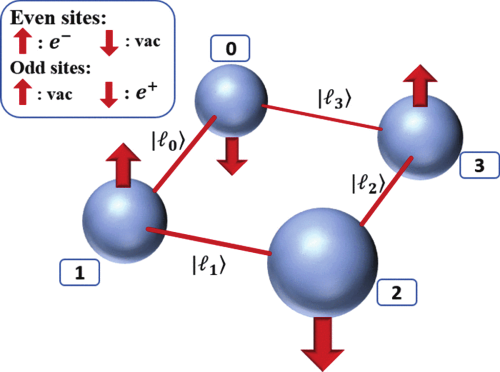
\includegraphics[width=10cm]{imgs/app3.png}
          };
        \end{tikzpicture}
      \end{block}
    \end{column} % End of the third column
  \end{columns} % End of all the columns in the poster
\end{frame} % End of the enclosing frame

\end{document}
